\documentclass[11pt, a4paper]{article}
\usepackage[margin=1in]{geometry}
  \usepackage{times}
  \usepackage{courier}
  \usepackage{multicol}
  \usepackage{hyperref}
  \usepackage{listings}
  \usepackage{color}
  % For code highlighting. Taken from
  % https://en.wikibooks.org/wiki/LaTeX/Source_Code_Listings
  \definecolor{mygreen}{rgb}{0,0.6,0}
  \definecolor{mygray}{rgb}{0.5,0.5,0.5}
  \definecolor{mymauve}{rgb}{0.58,0,0.82}
  \lstset{
    basicstyle=\footnotesize,        % the size of the fonts that are used for the code
    breakatwhitespace=false,         % sets if automatic breaks should only happen at whitespace
    breaklines=true,                 % sets automatic line breaking
    commentstyle=\color{mymauve},    % comment style
    keepspaces=true,                 % keeps spaces in text, useful for keeping indentation of code (possibly needs columns=flexible)
    keywordstyle=\color{blue},       % keyword style
    numbers=none,                    % where to put the line-numbers; possible values are (none, left, right)
    numbersep=5pt,                   % how far the line-numbers are from the code
    showspaces=false,                % show spaces everywhere adding particular underscores
    showstringspaces=false,
    numberstyle=\tiny\color{mygray}, % the style that is used for the line-numbers
    stringstyle=\color{mygreen},     % string literal style
    tabsize=2,                       % sets default tabsize to 2 spaces
  }
  
  
\usepackage[numbers,square]{natbib}
\bibliographystyle{unsrtnat}

\usepackage{parskip}
\setlength{\parindent}{0pt}

  \usepackage{graphicx}
  \usepackage[T1]{fontenc}
  \usepackage[utf8]{inputenc}
  \frenchspacing
  \setlength{\pdfpagewidth}{21.0cm}
  \setlength{\pdfpageheight}{29.7cm}
  \pdfinfo{
  /Title (Crazy, stupid, love.)
  /Author (Victor Chibotaru, Larissa Laich, Galina Peycheva, Ondrej Skopek)}
  %\setcounter{secnumdepth}{0}
  \newcommand{\TODO}[1]{\begin{center}\large\textbf{TODO:} #1\end{center}}
\begin{document}

\title{Crazy, stupid, love.}
\author{Victor Chibotaru\quad Larissa Laich\quad Galina Peycheva\quad Ondrej Skopek\\
  Team 5\\
  Department of Computer Science\\
  ETH Zurich\\
  Switzerland\\
  \texttt{\{viktorc, llaich, galinap, oskopek\}@ethz.ch}
}
\maketitle
\begin{abstract}
    Attempt to penetrate a company's internal employee registry to
    recover a girl's phone number. To do this, you have to overcome
    multiple layers of security.
	To get SSH access to the company's
    server, you need to first obtain user credentials using a server-side XXE
    vulnerability. Then, to obtain the first part of the admin's SSH password, you
    exploit a server-side template injection vulnerability in the
    admin's contact form, and obtain the second part of their password by
    reverse engineering a custom-made two-factor authentication app.
 	Using those secrets, you log in to the admin's server
    and get an encrypted ZIP file of the company's internal employee
    registry. Using a known-plaintext ZIP vulnerability, you
    decrypt and decompress the file, and get the phone number you lost!
\end{abstract}

%TODO:
% * Enhance mitigation part?
% * Clarify the steps and instructions.
%   * Screenshots?

\section{Backstory}

One day at PapperlaPub, you meet this amazing girl and start a long
conversation with her. You are super excited: Despite your computer
science background, you managed to get her phone number! The next
morning, when you sober up, you start thinking about your amazing
evening, and want to text her. Where did you put her phone number? After
desperately searching for hours, you realize that you've
probably lost it on your way home! What should you do now?

Fortunately, you remember that she works at Gügli. So you try to call
the company but the secretary tells you that she will not provide any
data about employees, and also will not forward any message to the girl.
You are very upset. How can anybody be that mean? Suddenly, it hits you.
The girl was complaining about their local sysadmin a lot. Should you
try to get the phone number by hacking into the Gügli system? It's a
long shot, but it's definitely worth a try!

\section{Requirements}

We will need two VMs:

\begin{enumerate}
  \item Client VM, with:
  \vspace{-0.5em}
  \begin{multicols}{2}
	\begin{itemize}
		\setlength\itemsep{-0.2em}
		\item Browser (or curl for the adventurous)
  		\item Java, JDGUI
  		\item nmap
  		\item nc
		\item pkcrack
  		\item Python
  		\item SSH client
  		\item A brute-force solution for SSH\\ (e.g. \mbox{THC-Hydra} or sshpass + bash)
	\end{itemize}
\end{multicols}

  \item Server VM (Linux, any version/distribution), with:
    \vspace{-0.5em}
  \begin{multicols}{2}
        \begin{itemize}
		\setlength\itemsep{-0.2em}
          \item Web server (Flask + uwsgi + Nginx)
          \item SSH daemon
          \item Python
          \item OpenSSL
        \end{itemize}
        \end{multicols}
\end{enumerate}



\section{Learning goal}

In practice, getting root access is a multistep process. Systems and
networks are protected on multiple levels. (Un)fortunately, each of the
steps often has several vulnerabilities. In our challenge, level:

\begin{enumerate}
  \item teaches you that
        \begin{enumerate}
          \item XML External Entity Injection (XXE, \citep{xxe}) is an easy to miss and easy to exploit vulnerability, which may lead to Server-Side Request Forgery (SSRF, \citep{ssrf}) and data leaks,
          \item one should disable XML's external entities processing if they are not needed,
          \item not sanitizing user input is a bad idea every time;
        \end{enumerate}

  \item teaches you that
        \begin{enumerate}
          \item there is such an attack as Server Side Template Injection (SSTI, \citep{ssti}),
          \item one should only use secure APIs and use them properly --- reinventing the wheel is a bad security practice,
          \item again: not sanitizing user input is a bad idea every time;
        \end{enumerate}

  \item teaches you that
        \begin{enumerate}
          \item even inside a secured system, protecting yourself and all other systems
                is still important,
          \item two factor authentication (2FA) is important, but also important to get right,
          \item implementing own cryptography is a bad idea in most cases,
          \item two factor authentication should resist brute-force attacks (ideally, use one-time tokens with a negligible probability of guessing);
        \end{enumerate}

  \item teaches you that
        \begin{enumerate}
          \item system administrators might not be the security gurus they pretend to be,
          \item ZIP archives might be vulnerable to Known-Plaintext Attacks (KPA, \citep{kpa}),
          \item storing your company's important details locally in an encrypted ZIP
                file is a very bad idea, even if only the administrator has access.
        \end{enumerate}

\end{enumerate}

\section{Mission}

Gain access to the company's employee registry data containing the
girl's lost number! The registry data is surely backed up in some folder on the server by the system administrator \ldots

\section{Mitigation}

\begin{description}
  \item[Step 1]~
  \begin{itemize}
	\item Thoroughly check and sanitize user input!
	\item For the XXE vulnerability --- disable the External Entities feature in your XML parser.
	\item Minimize the attack surface by not exposing such powerful tools like XML queries
        to users.
  \end{itemize}        
        
  \item[Step 2]~
	\begin{itemize}
	\item Thoroughly check and sanitize user input!
	\item For the SSTI vulnerability --- use the correct API provided by the template rendering engine.
	\item Do not leave debugging info lying around. 
    \item Never write down important passwords,
        at least in a way that is accessible online in any way.
	\end{itemize}
	
  \item[Step 3]~
  \begin{itemize}
  	\item Do not create your own and buggy software for two factor authentication.
  	\item Use trusted, proven, and updated versions of software.
  \end{itemize}    
        
  \item[Step 4]~
	\begin{itemize}
	\item Never store critically important information on servers accessible from the
        external network if access is not absolutely necessary.
     \item Do not store backups in password-protected ZIP files.
     \item Store unrelated data separately.
     \end{itemize}	  
\end{description}

\section{Type of challenge}

This is an online challenge.

\section{Category}

\begin{itemize}
  \item Penetration Testing
  \item Web Security
  \item Reverse Engineering
  \item Cryptography
\end{itemize}

\section{Hints}

We've decided that for such a big challenge three hints are not enough. That's
why we moved the hints to the \texttt{/hints} URL path of the web server
and made them more fine-grained.

\section{Step-by-step instructions}

\begin{figure}
    \begin{center}
    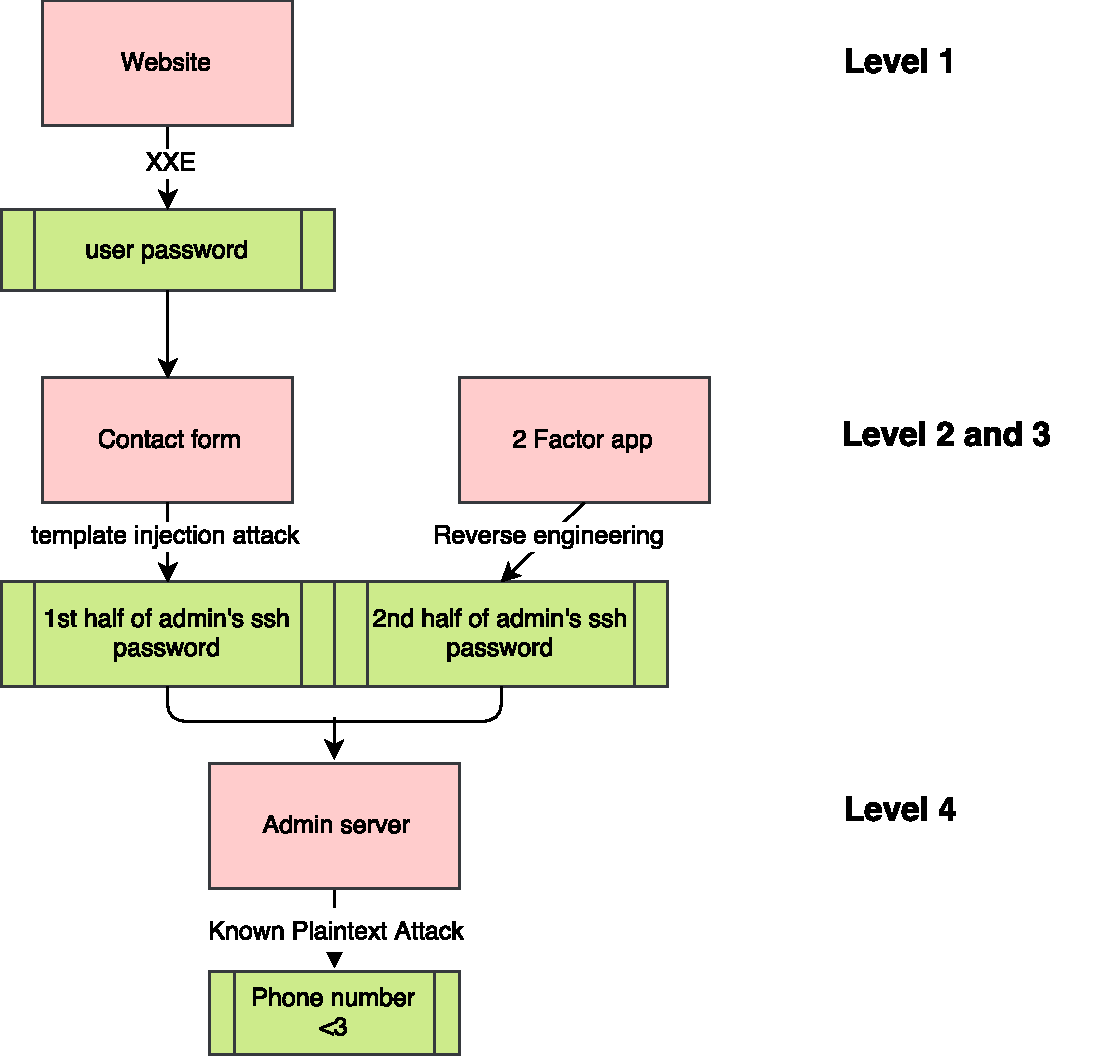
\includegraphics[width=0.65\textwidth]{images/diagram}
    \end{center}
    \caption{An overview of our challenge. The system's vulnerable components
    are displayed as red boxes and the obtained data in green boxes. The attacks
    to exploit the vulnerabilities are written on the edges.}
    \label{fig:diag}
\end{figure}

For a general overview of the different steps, see Figure \ref{fig:diag}.

\begin{enumerate}
  \item Do network reconnaissance.
  \item Find the Server VM, enumerate all the open ports using nmap, figure
        out which services are running for each of the ports.
  \item Get user access to the company's server.
        \begin{enumerate}
          \item Use an XXE exploit to attack the service for listing users and their public keys.
            The service will accept ``smart'' queries written in XML to filter out
            the search results, but luckily for you, the parser is
            vulnerable to XXE. Thus, it is possible to extract files
            from the server. The paths to the web application's source files
            are ``accidentally'' inserted into the query response web page
            as debug output that someone forgot to remove.
          \item To exploit the vulnerability use the following vector, which
            dumps the contents of the file located at provided path:
            \lstinputlisting[language=XML]{exploits/xxe_exploit.txt}
          \item Use the exploit to dump the \texttt{\_\_init.py\_\_}
            (the path to it is provided as "debug info" in the web page).
            The database file is unfortunately not obtainable using this vulnerability,
            as it contains a null character.
          \item Read the dumped file and notice that it imports another
            Python module called \texttt{models}.
          \item Using the same exploit and elementary Python knowledge
            (the \texttt{models} module source file is very likely in the
            same folder and named \texttt{models.py}), dump the \texttt{models.py} file.
          \item Read the file and notice ``accidentally'' forgotten usernames
            and password hashes.
          \item Recover the passwords from their hashes using a rainbow table, e.g.~John the Ripper or
            a website such as:
            \begin{center} \url{https://crackstation.net} \end{center}
        \end{enumerate}

      \item Steal the first half of admin's SSH password.
        \begin{enumerate}
          \item The company's admin contact form is vulnerable to multiple
            injection attacks (including reflected Cross-Site Scripting (XSS, \citep{xss}) and SSTI). Our intention
            is to make students first try the obvious XSS vectors and realize
            that they are not working because the admin wrote a server-side script,
            which generates automatic replies to users' queries, and is not aware of
            JavaScript at all.
          \item The second attack vector would be one against the template
            rendering engine. Here's a possible exploit for it:
            \lstinputlisting[language=Python]{exploits/flask_exploit.txt}
            This exploit starts a remote shell accessible at port 8000.
          \item Use \texttt{nc gugli 8000} to connect to the shell and explore the web application
            source files.
          \item Find the previously unobtainable \texttt{view.py} file
           (the file was not readable with the previous XXE exploit).
          \item Find the first half of admin's SSH password in the file.
        \end{enumerate}

      \item Steal the second half of admin's SSH password.
        \begin{enumerate}
          \item Find the 2FA app in the menu and download it.
          \item Use a java decompiler and check out the algorithm.
            Understand that there's no way to recover the needed secret, but
            the algorithm returns only three decimal digits!
          \item Brute-force the obtained password appended with a 2FA token
            using THC-Hydra or \texttt{ssh} and \texttt{sshpass} combined with elementary \texttt{bash} scripting: \lstinputlisting[language=Bash]{exploits/ssh_brute_force.txt}
        \end{enumerate}

      \item Recover the girl's number from the encrypted database.
        \begin{enumerate}
          \item Find the \texttt{\textasciitilde/database\_backup/backup.zip} file.
          \item Read through the \texttt{contents.txt} file next to it.
            Tt describes the contents of the ZIP archive.
          \item Understand that the encrypted archive contains the file.
          \item Realize that a Known-Plaintext Attack is possible.
          \item Use, for example, PkCrack:\\
            \texttt{pkcrack -p contents.txt -e contents.txt -P contents.zip \textbackslash}\\
            \texttt{-C backup.zip -d output.zip}\\
            Important note: \texttt{contents.zip} should be created with the same \texttt{zip}
            options as the original \texttt{backup.zip}. The options are stated
            in the \texttt{contents.txt} file. The archive should be generated on the
            \textbf{server} machine in order to use the same ZIP version,
            but can be decrypted on the client VM.
          \item Find the girl's number in the DB!
        \end{enumerate}

\end{enumerate}


\section{Implementation}

\subsection{Network}
  The network consists of two VMs with statically allocated IP addresses:
  \begin{itemize}
    \item Server: \texttt{192.168.0.1} (with hostname \texttt{gugli} set on client VM)
    \item Client: \texttt{192.168.0.2}
  \end{itemize}
  Both of the VMs have "internal network" VirtualBox network adapters. No other
  special network setup is required, so deploying the challenge in some other
  environment should be straightforward. Just make sure to statically set the
  server's IP address and provide it to the client.

  The client VM  has an additional "NAT" adapter for internet access.
  
\subsection{Server}
  The server is a Debian 9 VM. It runs an Nginx + uwsgi + Flask web server.
  There are two user accounts available for interactive login (via SSH too):
  \begin{itemize}
    \item \texttt{root:gtavibkznsseauu}
    \item \texttt{bestadminever:ilovekittens988}
  \end{itemize}

  We took care to protect the server against DOS attacks from evil students (in
  case the challenge gets deployed to a platform like Hacking Lab):
  \begin{itemize}
    \item None of the accounts on the server has \texttt{sudo} privileges (except root).
    \item All the important for the challenges files are owned by root and only
      readable by corresponding users. The only exception are the files contained
      in the \texttt{/home/www-data/webapp\_writable} folder. Those are the
      Linux FIFO between Nginx and uwsgi, and the logs of the Flask server. We could
      not come up with a solution for those files. In case they get deleted
      all that needs to be done to restore the server's state is:
      \texttt{systemctl restart webapp.service} under root.
  \end{itemize}

  Another risk is students getting root access by exploiting some fresh Linux
  vulnerabilities, but we see no way of defending against ahead of time.

\subsection{Client}
  The client is a Ubuntu 16.04 VM. It has all the necessary tools installed in
  \texttt{/home/hacker/tools} folder.

  It also has the \texttt{gugli} hostname and corresponding IP address added in \texttt{/etc/hosts}. Other than
  that it, is a typical out-of-the-box Ubuntu distribution and could easily be replaced
  by any other distribution (i.e.~the Hacking Lab Client VM).

\subsection{Local challenge setup}

\begin{enumerate}
    \item Import the two VMs into VirtualBox.
    \item Start the Server VM (headless).
    \item Login to the Client VM using \texttt{hacker:hacker}.
    \item The server is accessible at the IP \texttt{192.168.0.1} or DNS name \texttt{gugli}
    from the Client VM.
\end{enumerate}

\bibliography{biblio}

\end{document}
